% !TEX TS-program = pdflatex
% !TEX encoding = UTF-8 Unicode

% This file is a template using the "beamer" package to create slides for a talk or presentation
% - Talk at a conference/colloquium.
% - Talk length is about 20min.
% - Style is ornate.

% MODIFIED by Jonathan Kew, 2008-07-06
% The header comments and encoding in this file were modified for inclusion with TeXworks.
% The content is otherwise unchanged from the original distributed with the beamer package.

\documentclass{beamer}


% Copyright 2004 by Till Tantau <tantau@users.sourceforge.net>.
%
% In principle, this file can be redistributed and/or modified under
% the terms of the GNU Public License, version 2.
%
% However, this file is supposed to be a template to be modified
% for your own needs. For this reason, if you use this file as a
% template and not specifically distribute it as part of a another
% package/program, I grant the extra permission to freely copy and
% modify this file as you see fit and even to delete this copyright
% notice. 


\mode<presentation>
{
  \usetheme{Warsaw}
  % or ...

  \setbeamercovered{transparent}
  % or whatever (possibly just delete it)
}


\usepackage[english]{babel}
% or whatever

\usepackage[utf8]{inputenc}
% or whatever

\usepackage{times}
\usepackage[T1]{fontenc}
% Or whatever. Note that the encoding and the font should match. If T1
% does not look nice, try deleting the line with the fontenc.
 \newcommand{\abs}[1]{\left|{#1}\right|}
 \newcommand{\av}[1]{\left\langle #1 \right\rangle}
 
  \newcommand{\br}[1]{\langle #1|}
  \newcommand{\ke}[1]{|#1\rangle}
  \newcommand{\bk}[2]{\langle #1|#2\rangle}
  \newcommand{\kb}[2]{\ke{#1}\br{#2}}
  \newcommand{\var}[2]{\langle #1|#2\rangle} 
  \newcommand{\ov}[2]{\abs{\var{#1}{#2}}^2}
\newcommand{\td}[1]{\widetilde{#1}}

%\title[Short Paper Title] % (optional, use only with long paper titles)
%{Second Examination}

\title
{Optimal Measurement Tasks and Their Physical Realizations}

\author[Vadim Yerokhin] % (optional, use only with lots of authors)
{Vadim Yerokhin }
% - Give the names in the same order as the appear in the paper.
% - Use the \inst{?} command only if the authors have different
%   affiliation.

% - Use the \inst command only if there are several affiliations.
% - Keep it simple, no one is interested in your street address.

\date[CFP 2003] % (optional, should be abbreviation of conference name)
{Hunter College, August 25th 2015 }
% - Either use conference name or its abbreviation.
% - Not really informative to the audience, more for people (including
%   yourself) who are reading the slides online


% If you have a file called "university-logo-filename.xxx", where xxx
% is a graphic format that can be processed by latex or pdflatex,
% resp., then you can add a logo as follows:

% \pgfdeclareimage[height=0.5cm]{university-logo}{university-logo-filename}
% \logo{\pgfuseimage{university-logo}}



% Delete this, if you do not want the table of contents to pop up at
% the beginning of each subsection:
\AtBeginSubsection[]
{
  \begin{frame}<beamer>{Outline}
    \tableofcontents[currentsection,currentsubsection]
  \end{frame}
}


% If you wish to uncover everything in a step-wise fashion, uncomment
% the following command: 

%\beamerdefaultoverlayspecification{<+->}


\begin{document}

\begin{frame}
  \titlepage
\end{frame}

\begin{frame}{Outline}
  \tableofcontents[pausesections]
  % You might wish to add the option [pausesections]
\end{frame}


% Structuring a talk is a difficult task and the following structure
% may not be suitable. Here are some rules that apply for this
% solution: 

% - Exactly two or three sections (other than the summary).
% - At *most* three subsections per section.
% - Talk about 30s to 2min per frame. So there should be between about
%   15 and 30 frames, all told.

% - A conference audience is likely to know very little of what you
%   are going to talk about. So *simplify*!
% - In a 20min talk, getting the main ideas across is hard
%   enough. Leave out details, even if it means being less precise than
%   you think necessary.
% - If you omit details that are vital to the proof/implementation,
%   just say so once. Everybody will be happy with that.

%%%%%%%%%%%%%%%%%%%%%%%%%%%%%%%%%%%%%%%%%%%%%%%%
%%%%%%%%%%%%%%%%%%%%%%%%%%%%%%%%%%%%%%%%%%%%%%%%
\section{Introduction}
\subsection{Information Theory}
\begin{frame}{Motivation}
\begin{itemize}
\item
Classical bits versus quantum bits: instead of just a 0 or 1, quantum bits can maintain a superposition state of both.

\item
Quantum computing: Shor's algorithm allows cracking of modern communications security based on prime decomposition.

\item
Quantum communication: B92 protocol allows for completely secure communication.
\end{itemize}
\end{frame}
%%%%%%%%%%%%%%%%%%%%%%%%%%%%%%%%%%%%%%%%%%%%%%%%
%%%%%%%%%%%%%%%%%%%%%%%%%%%%%%%%%%%%%%%%%%%%%%%%
\begin{frame}{Our Games}
\begin{itemize}
\item
Someone prepares one of two different pure states $\ke {\psi_i} = \alpha_i \ke 0 +  \beta_i \ke 1$
for $i = 1,2$.

\item
Each state's occurrence has a different likelihood $\eta_i$ that sum to 1: $\eta_1+\eta_2 =1$.

\item
One particle (state) is sent at a time.  Our job is to:
\begin{itemize}
\item
 Guess as best we can which state was sent (discrimination)
\item Make the state more orthogonal to its complement (separation)
\item
Make copies of the input state (cloning)

\end{itemize}

\end{itemize}

\end{frame}

%%%%%%%%%%%%%%%%%%%%%%%%%%%%%%%%%%%%%%%%%%%%%%%%
%%%%%%%%%%%%%%%%%%%%%%%%%%%%%%%%%%%%%%%%%%%%%%%%
\begin{frame}{Neumark's theorem}
\begin{itemize}
\item
The unitary time evolution of a pure system evolving with a pure ancilla can be described as
\[U(\ke {\psi_A} \otimes \ke {\phi_B}) = \sum_i A_i \ke {\psi_A} \otimes \ke {i_B}.\]
using the  Kraus operators $A_i$ such that $\sum A^\dagger_i A_i = \sum \Pi_i = I$.
The $\Pi_i$'s represent different measurement outcomes.

\item
The other is simply as a unitary acting on a pure state $\psi$ to make state $\phi$, as in $U\ke \psi = \ke \phi$.
\end{itemize}
\end{frame}
%%%%%%%%%%%%%%%%%%%%%%%%%%%%%%%%%%%%%%%%%%%%%%%%
%%%%%%%%%%%%%%%%%%%%%%%%%%%%%%%%%%%%%%%%%%%%%%%%
\subsection{Pure State Discrimination Strategies}

\begin{frame}{No-go}
If perfect discrimination were possible we would write it as
\[\Pi_1 \ke {\psi_2} = 0,\]
\[\Pi_2 \ke {\psi_1} = 0.\]
Then using $\Pi_1 + \Pi_2 = I$ and the inner product of these equations, we get a contradictory result:
\[0= \br{\psi_1} \Pi_1 + \Pi_2 \ke {\psi_2} = \bk{\psi_1}{\psi_2} \]
 Since the two constraints of measurement,
orthogonality of the measurement vectors to the states and their spanning the space proved incompatible we must give up one of these two
functions in order to perform a physical measurement.
\end{frame}
%%%%%%%%%%%%%%%%%%%%%%%%%%%%%%%%%%%%%%%%%%%%%%%%
%%%%%%%%%%%%%%%%%%%%%%%%%%%%%%%%%%%%%%%%%%%%%%%%
\begin{frame}{Minimum Error Discrimination (ME)}
\begin{itemize}
\item
	Two orthogonal projectors, each clicks for a state.
\item
	There is a success rate and an error rate if the states are not orthogonal:
\[ P_s =\eta_1 \br {\psi_1} \Pi_1\ke {\psi_1} + \eta_2 \br {\psi_2} \Pi_2\ke {\psi_2},\]
\[ P_e = \eta_1 \br {\psi_1} \Pi_2\ke {\psi_1} + \eta_2 \br {\psi_2} \Pi_1\ke {\psi_2}.\]

\item
	The minimum error rate for pure states is achieved at the Helstrom bound:
\[P_E = \frac{1}{2}(1- \sqrt{1-4 \eta_1 \eta_2 \ov{\psi_1}{\psi_2}}).\]
\end{itemize}
\end{frame}

%%%%%%%%%%%%%%%%%%%%%%%%%%%%%%%%%%%%%%%%%%%%%%%%
%%%%%%%%%%%%%%%%%%%%%%%%%%%%%%%%%%%%%%%%%%%%%%%%
\begin{frame}{Unambiguous State Discrimination (UD)}



\begin{itemize}
\item
	Make the measurement operators orthogonal to the states that we don't want to measure.

\item
	Since they are no longer orthogonal to each other they don't sum to the identity. A third, inconclusive outcome is necessary.
\item
	The detector corresponding to the inconclusive outcome we call $\Pi_0$.

\item
	The failure probability we call Q:

\[Q =  \eta_1 \br {\psi_1} \Pi_0\ke {\psi_1} + \eta_2 \br {\psi_2} \Pi_0\ke {\psi_2}\]

\item
$ Q_0 = 2 \sqrt{\eta_1\eta_2} cos \theta$  is the failure rate that corresponds to the best measurement.
\end{itemize}

\end{frame}
%%%%%%%%%%%%%%%%%%%%%%%%%%%%%%%%%%%%%%%%%%%%%%%%
%%%%%%%%%%%%%%%%%%%%%%%%%%%%%%%%%%%%%%%%%%%%%%%%

\begin{frame}{Intermediate Discrimination (IM)}
\begin{figure}[th]
\centering
$%
\begin{array}{c}
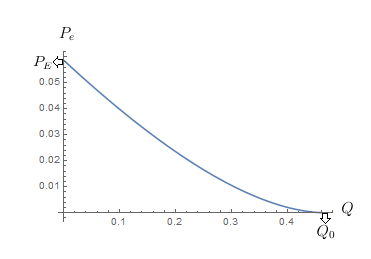
\includegraphics[height=6 cm]{IM.png} \\

\end{array}%
$%

\label{fig:Graphs}
\end{figure}

\end{frame}
%%%%%%%%%%%%%%%%%%%%%%%%%%%%%%%%%%%%%%%%%%%%%%%%
%%%%%%%%%%%%%%%%%%%%%%%%%%%%%%%%%%%%%%%%%%%%%%%%
\begin{frame}{Lagrange Multipliers method}
We can cast the problem via Neumark's theorem as
\begin{eqnarray*}
U \ke {\psi_1}= \sqrt{p_1} \ke 1 + \sqrt{r_1} \ke 2 + \sqrt{q_1} \ke 0, \\
U |\psi_2 \rangle = \sqrt{r_2} \ke 1 + \sqrt{p_2} \ke 2 + \sqrt{q_2} \ke 0.
\end{eqnarray*}

The inner product of these two equations is useful. We call it the unitarity constraint:
\[s = \langle\psi_1|\psi_2\rangle\ = \sqrt{p_1 r_2} + \sqrt{p_2 r_1} + \sqrt{q_1 q_2}.\]
\end{frame}
%%%%%%%%%%%%%%%%%%%%%%%%%%%%%%%%%%%%%%%%%%%%%%%%
%%%%%%%%%%%%%%%%%%%%%%%%%%%%%%%%%%%%%%%%%%%%%%%%
\begin{frame}
We now use the Lagrange multiplier method to minimize $P_e$ subject to the inner-product constraint and fixed failure rate Q.
\[F_e = \eta_1 r_1 + \eta_2 r_2 + \lambda (s - \rm Unitarity\hspace{.1 cm}Constraint ).\]
A lot of algebra gives us the optimal individual error rates as:
\begin{equation}
r_{i}  =\frac{1}{4\eta_i}\left[\left(2 \eta_i-Q\right)-\frac{\left(2 \eta_i-Q\right)\left(1-Q\right)-(Q_{o}-Q)^{2}}{\sqrt{(1-Q)^{2}-(Q-Q_{o})^{2}}}\right],\label{eq:r_i}
\end{equation}
 and the total error rate as
\[ P_e = \frac{1}{2} \left[1 - Q -\sqrt{(1-Q)^2 - (Q-Q_0)^2}\right].\]
\end{frame}

%%%%%%%%%%%%%%%%%%%%%%%%%%%%%%%%%%%%%%%%%%%%%%%%
%%%%%%%%%%%%%%%%%%%%%%%%%%%%%%%%%%%%%%%%%%%%%%%%
\begin{frame}
We've solved some state discrimination problems involving mixed states but we've presented the results before so we move on to other,
more interesting topics!
\end{frame}

\begin{frame}
We can consider operations such as UD or IM as two-step measurements:
\begin{itemize}
\item
In the first step we probabilistically separate the states.  
\item
In the second step, if the first was successful, orthogonal detection operators (ME) discriminate the states.
\end{itemize}
\[\]
What if we only wanted to perform the first step? 
\end{frame}

%%%%%%%%%%%%%%%%%%%%%%%%%%%%%%%5
%%%%%%%%%%%%%%%%%%%%%%%%%%%%%%%%%%
%%%%%%%%%%%%%%%%%%%%%%%%%%%%%%%5
%%%%%%%%%%%%%%%%%%%%%%%%%%%%%%%%%%
%%%%%%%%%%%%%%%%%%%%%%%%%%%%%%%5
%%%%%%%%%%%%%%%%%%%%%%%%%%%%%%%%%%
\section{Pure State Separation}
\begin{frame}
We want to make the pure states $\psi_i$ probabilistically more distinguishable, via
equations
\begin{eqnarray*}
U|\psi_{1}\rangle|0\rangle & = & \sqrt{p_{1}}|\phi_{1}\rangle|1\rangle+\sqrt{q_{1}}\ke 0,\nonumber \\
U|\psi_{2}\rangle|0\rangle & = & \sqrt{p_{2}}|\phi_{2}\rangle|1\rangle+\sqrt{q_{2}}\ke 0.
\end{eqnarray*}
Here the inner product equation is $s = \sqrt{p_1 p_2} s' + \sqrt{q_1 q_2}$ where $s' = \bk{\phi_1}{\phi_2}$ and $p_i + q_i =1$.

Our goal is to maximize the separation $s'$ for a fixed failure rate $Q = \eta_1 q_1 + \eta_2 q_2$ or alternately to minimize Q for a fixed $s'$.

We can easily derive the solution for equal priors as $p = (1-s)/(1-s')$. The general solution is not trivial.
\end{frame}
%%%%%%%%%%%%%%%%%%%%%%%%%%%%%%%5
%%%%%%%%%%%%%%%%%%%%%%%%%%%%%%%%%%
\begin{frame}
A particularly attractive geometric formulation of this constraint comes from
choosing the change of variables 
$u\equiv\sqrt{q_{1}q_{2}},\hspace{0.3cm}v\equiv\frac{1}{2}\left(q_{1}+q_{2}\right)$.
\begin{itemize}
\item
The unitarity constraint becomes the parabola $v={1+u^2\over2}-{(u-s)^2\over2s'^2}$.
\item
The failure rate curve becomes the parametrized ellipse
%
\begin{eqnarray}
u&=&{Q\over\sqrt{1-\Delta^2}}\cos\theta',\nonumber\\
v&=&{Q\over1-\Delta^2}+{Q\Delta\over1-\Delta^2}\sin\theta',
\end{eqnarray}
\end{itemize}
where $\Delta = \eta_2 - \eta_1$,
The optimality condition is the tangency of the ellipse and parabola. We are able to derive all bounds parametrically.
\end{frame}
%%%%%%%%%%%%%%%%%%%%%%%%%%%%%%%5
%%%%%%%%%%%%%%%%%%%%%%%%%%%%%%%%%%
\begin{frame}
\begin{figure}[th]
\centering
$%
\begin{array}{c}
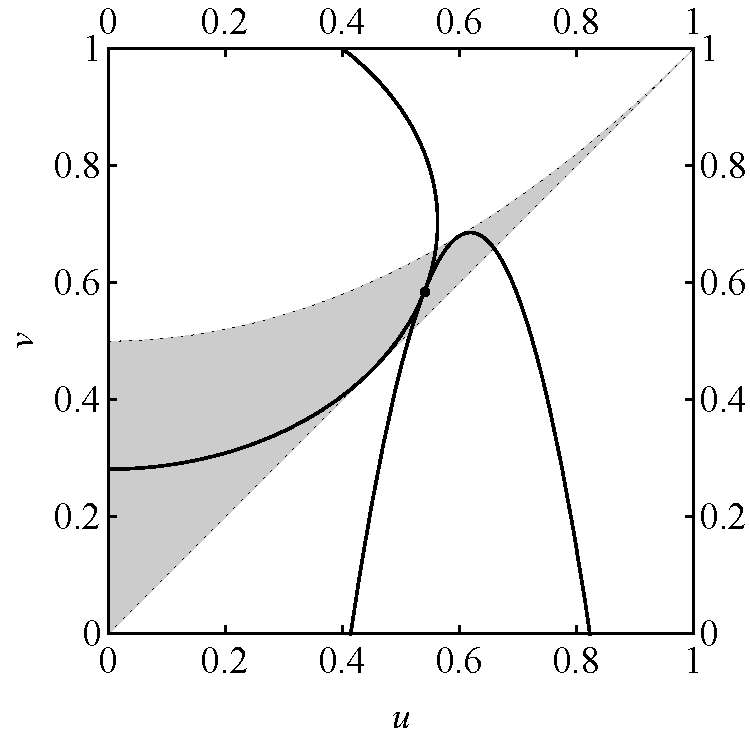
\includegraphics[height=7 cm]{Figures_SEPvedit.pdf} \\

\end{array}%
$%

\label{fig:Graphs}
\end{figure}


\end{frame}


%%%%%%%%%%%%%%%%%%%%%%%%%%%%%%%5
%%%%%%%%%%%%%%%%%%%%%%%%%%%%%%%%%%
%%%%%%%%%%%%%%%%%%%%%%%%%%%%%%%5
%%%%%%%%%%%%%%%%%%%%%%%%%%%%%%%%%%
%%%%%%%%%%%%%%%%%%%%%%%%%%%%%%%5
%%%%%%%%%%%%%%%%%%%%%%%%%%%%%%%%%%
\section{Cloning Pure States}

\begin{frame}{No-go}
Suppose we wrote the equations describing the unitary that cloned one of two input pure states $\psi_i$ with
a-priori probabilities $\eta_i$ for $i = 1,2$.  If we could perform this measurement perfectly we would write
\begin{eqnarray}
U\ke{\psi_1}\ke 0 = \ke{\psi_1}\ke{\psi_1},\\
U\ke{\psi_2}\ke 0 = \ke{\psi_2}\ke{\psi_2}.
\end{eqnarray}
However, taking the inner product of the two equations we find $\bk{\psi_1}{\psi_2} = \bk{\psi_1}{\psi_2}^2$,
restricting the functionality of this unitary to the trivial cases when the two states are orthogonal or identical.
Therefore there does not exist in general a unitary to perform this ideal cloning task.  As with state discrimination, 
we must choose a figure of merit to maximize.
\end{frame}
%%%%%%%%%%%%%%%%%%%%%%%%%%%%%%%5
%%%%%%%%%%%%%%%%%%%%%%%%%%%%%%%%%%%%%%%%%%%%%%%%%%%%%%%%%%%%%%%%%5
%%%%%%%%%%%%%%%%%%%%%%%%%%%%%%%%%%
\subsection{Deterministic Approximate Cloning}
\begin{frame}
The 'ME' cloning method makes $n$ imperfect copies from $m$ copies of one of two input states.
The unitary representation of this transformation is
\begin{eqnarray*}
U \ke{\psi_1}^m\ke 0  = \ke {\phi_1}\\
U \ke{\psi_2}^m\ke 0  = \ke {\phi_2}
\end{eqnarray*}
Where given the fidelities $F_i = |\bk{\psi_i^n}{\phi_i}|^2$ we want to maximize is the average global fidelity
\[F = \eta_1 F_1 +\eta_2 F_2.\]
The optimal fidelity is
\[F = \frac{1}{2}( 1 + \sqrt{1-  4 \eta_1 \eta_2 \sin^2 \alpha}).\]
where $\alpha = \theta -\phi$, the difference between initial and final overlap angles and $\phi = \arccos \left[ (\cos \theta)^{m}\right]$.
\end{frame}
%%%%%%%%%%%%%%%%%%%%%%%%%%%%%%%5
%%%%%%%%%%%%%%%%%%%%%%%%%%%%%%%%%%%%%%%%%%%%%%%%%%%%%%%%%%%%%%%%%5
%%%%%%%%%%%%%%%%%%%%%%%%%%%%%%%%%%
\subsection{Probabilistic Exact Cloning}
\begin{frame}
Here we take the 'unambiguous' method to solving the problem and sometimes make perfect clones.  We consider $m$ input states turned into $n$ output states.
\begin{equation*}
U|\psi^m_i\rangle|0\rangle= \sqrt{p_i}|\psi^n_i\rangle|1\rangle +\sqrt q_i |\Phi\rangle |0\rangle,\quad i=1,2. \label{Ui}
\end{equation*}

The overlap equation now reads 
\[s^m = \bk {\psi_1^m}{\psi_2^m} = \sqrt{p_1 p_2} \bk {\psi_1^n}{\psi_2^n}  + \sqrt{q_1 q_2} =\sqrt{p_1 p_2} s^n+ \sqrt{q_1 q_2}.\]

If at this point you think this equation looks remarkably similar to everything else, you'd be right. But particularly to the separation
 unitarity condition with $s \rightarrow s^M$,$s' \rightarrow s^N$.  We can use that solution but we have another attractive option.
\end{frame}


%%%%%%%%%%%%%%%%%%%%%%%%%%%%%%%5
%%%%%%%%%%%%%%%%%%%%%%%%%%%%%%%%%%%%%%%%%%%%%%%%%%%%%%%%%%%%%%%%%5
\begin{frame}{Geometric Picture}
Suppose we are given the unitary curve
\[s^m=\sqrt{p_1 p_2} s^n+ \sqrt{q_1 q_2}\]
\href{file:///C:/Users/Vadim/Documents/work/Final exam/manipulateUnitaryCondition.swf}{This clip} shows the unitarity curves for different initial overlaps 
in the $q_1$ vs $q_2$ coordinate system.

 We want to minimize the failure rate 
\[q_2= \frac{Q}{1- \eta_1} -  \frac{\eta_1}{1- \eta_1} q_1 .\] 
These two equations appear as a complex curve and a straight line.  To satisfy both conditions means the curves must intersect.
It can be proven that tangency is the requirement. 
\end{frame}

%%%%%%%%%%%%%%%%%%%%%%%%%%%%%%%5
%%%%%%%%%%%%%%%%%%%%%%%%%%%%%%%%%%%%%%%%%%%%%%%%%%%%%%%%%%%%%%%%%5
\begin{frame}
\begin{figure}[t]
\centering
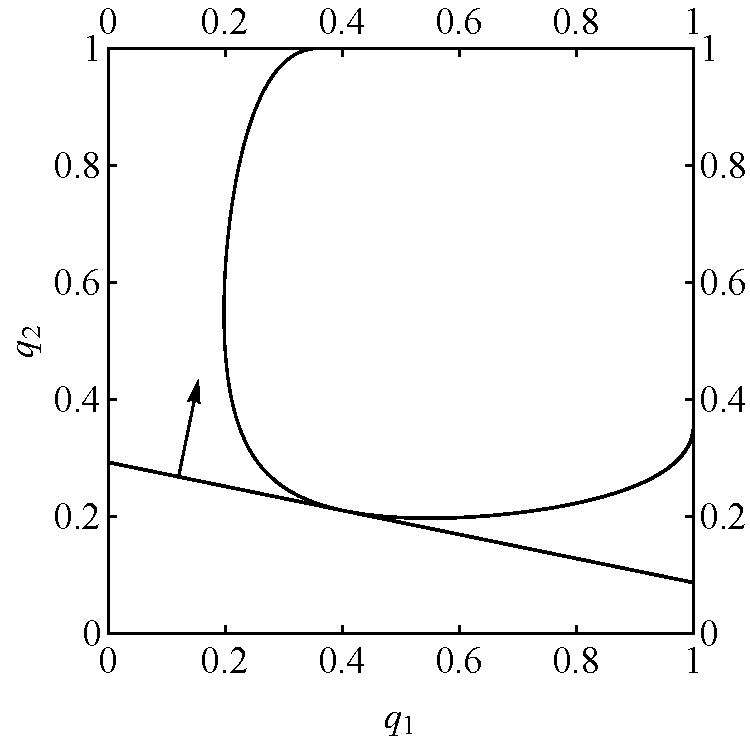
\includegraphics[width=14em]{Figures_CLONEvedit.pdf}
%
\caption{ The figure shows the overlap constraint and the optimal straight segment \mbox{$Q=\eta_1 q_1+\eta_2 q_2$} and its normal vector~$(\eta_1,\eta_2)$. Plotted for  $s = 0.6$, $\eta_1=0.17$, $\eta_2=0.83$ and~$Q=0.24$.}
\label{fig:1}
\end{figure}
\end{frame}
%%%%%%%%%%%%%%%%%%%%%%%%%%%%%%%5
%%%%%%%%%%%%%%%%%%%%%%%%%%%%%%%%%%%%%%%%%%%%%%%%%%%%%%%%%%%%%%%%%5
\begin{frame}{Parametrization}
We use the change of variables $\sqrt{q_i} = \sin \theta_i$ then $x = cos(\theta_1 + \theta_2)$, $y = (cos\theta_1 -\theta_2)$ to write the unitary constraint as
$2s^m=(1+s^n)y-(1-s^n)x $ where 
\[x=\frac{1-(1+s^n)t}{s^{n-m}},\qquad y=\frac{1-(1-s^n)t}{s^{n-m}}\]
for the range of values
\[t_{-1}=\frac{1-s^{n-m}}{1-s^n} \leq t \leq \frac{1-s^{2(n-m)}}{1-s^{2n}} = 
t_0.\]
We write the failure rates as
\begin{equation}
q_i=\frac{1-xy-(-1)^i\sqrt{1-x^2}\sqrt{1-y^2}}{2}.
\end{equation}
\end{frame}
%%%%%%%%%%%%%%%%%%%%%%%%%%%%%%%5
%%%%%%%%%%%%%%%%%%%%%%%%%%%%%%%%%%%%%%%%%%%%%%%%%%%%%%%%%%%%%%%%%5
\begin{frame}{Optimization}
We characterize our result by expressing the necessery a-priori $\eta_i$ as a function of $t$ for any point on the unitary curve.  Then we can solve for the minimum $Q$ using this value.  These equations take the form
\begin{equation*}
\eta_1=\frac{q'_2}{q'_2-q'_1},\;\; Q_{\rm min}=\frac{q'_2 q_1-q'_1 q_2}{q'_2-q'_1},
\label{main}
\end{equation*}
where the derivative of $q$ is
\begin{equation}
q'_i=\frac{\sqrt{q_i(1-q_i)}}{s^{n-m}}\left\{\frac{1+s^n}{\sqrt{1-x^2}}-(-1)^i\frac{1-s^n}{\sqrt{1-y^2}}\right\}.
\end{equation}
\end{frame}

%%%%%%%%%%%%%%%%%%%%%%%%%%%%%%%5
%%%%%%%%%%%%%%%%%%%%%%%%%%%%%%%%%%%%%%%%%%%%%%%%%%%%%%%%%%%%%%%%%5
\begin{frame}{Relation to State Discrimination}
Optimal cloning is always more successful than discrimination, though this difference decreases with more clones.  In the limit $n \rightarrow \infty$ there is perfect agreement.
In geometric terms, the unitary curve $s^m=\sqrt{p_1 p_2} s^n+ \sqrt{q_1 q_2}$ collapses onto the hyperbola $s^m =  \sqrt{q_1 q_2}$, which is the constraint for 
UD state discrimination.  Therefore the limiting solution to our cloning procedure is unambiguous discrimination.
\end{frame}
%%%%%%%%%%%%%%%%%%%%%%%%%%%%%%%5
%%%%%%%%%%%%%%%%%%%%%%%%%%%%%%%%%%%%%%%%%%%%%%%%%%%%%%%%%%%%%%%%%5
\begin{frame}
\begin{figure}[ht]
$%
\begin{array}{c}
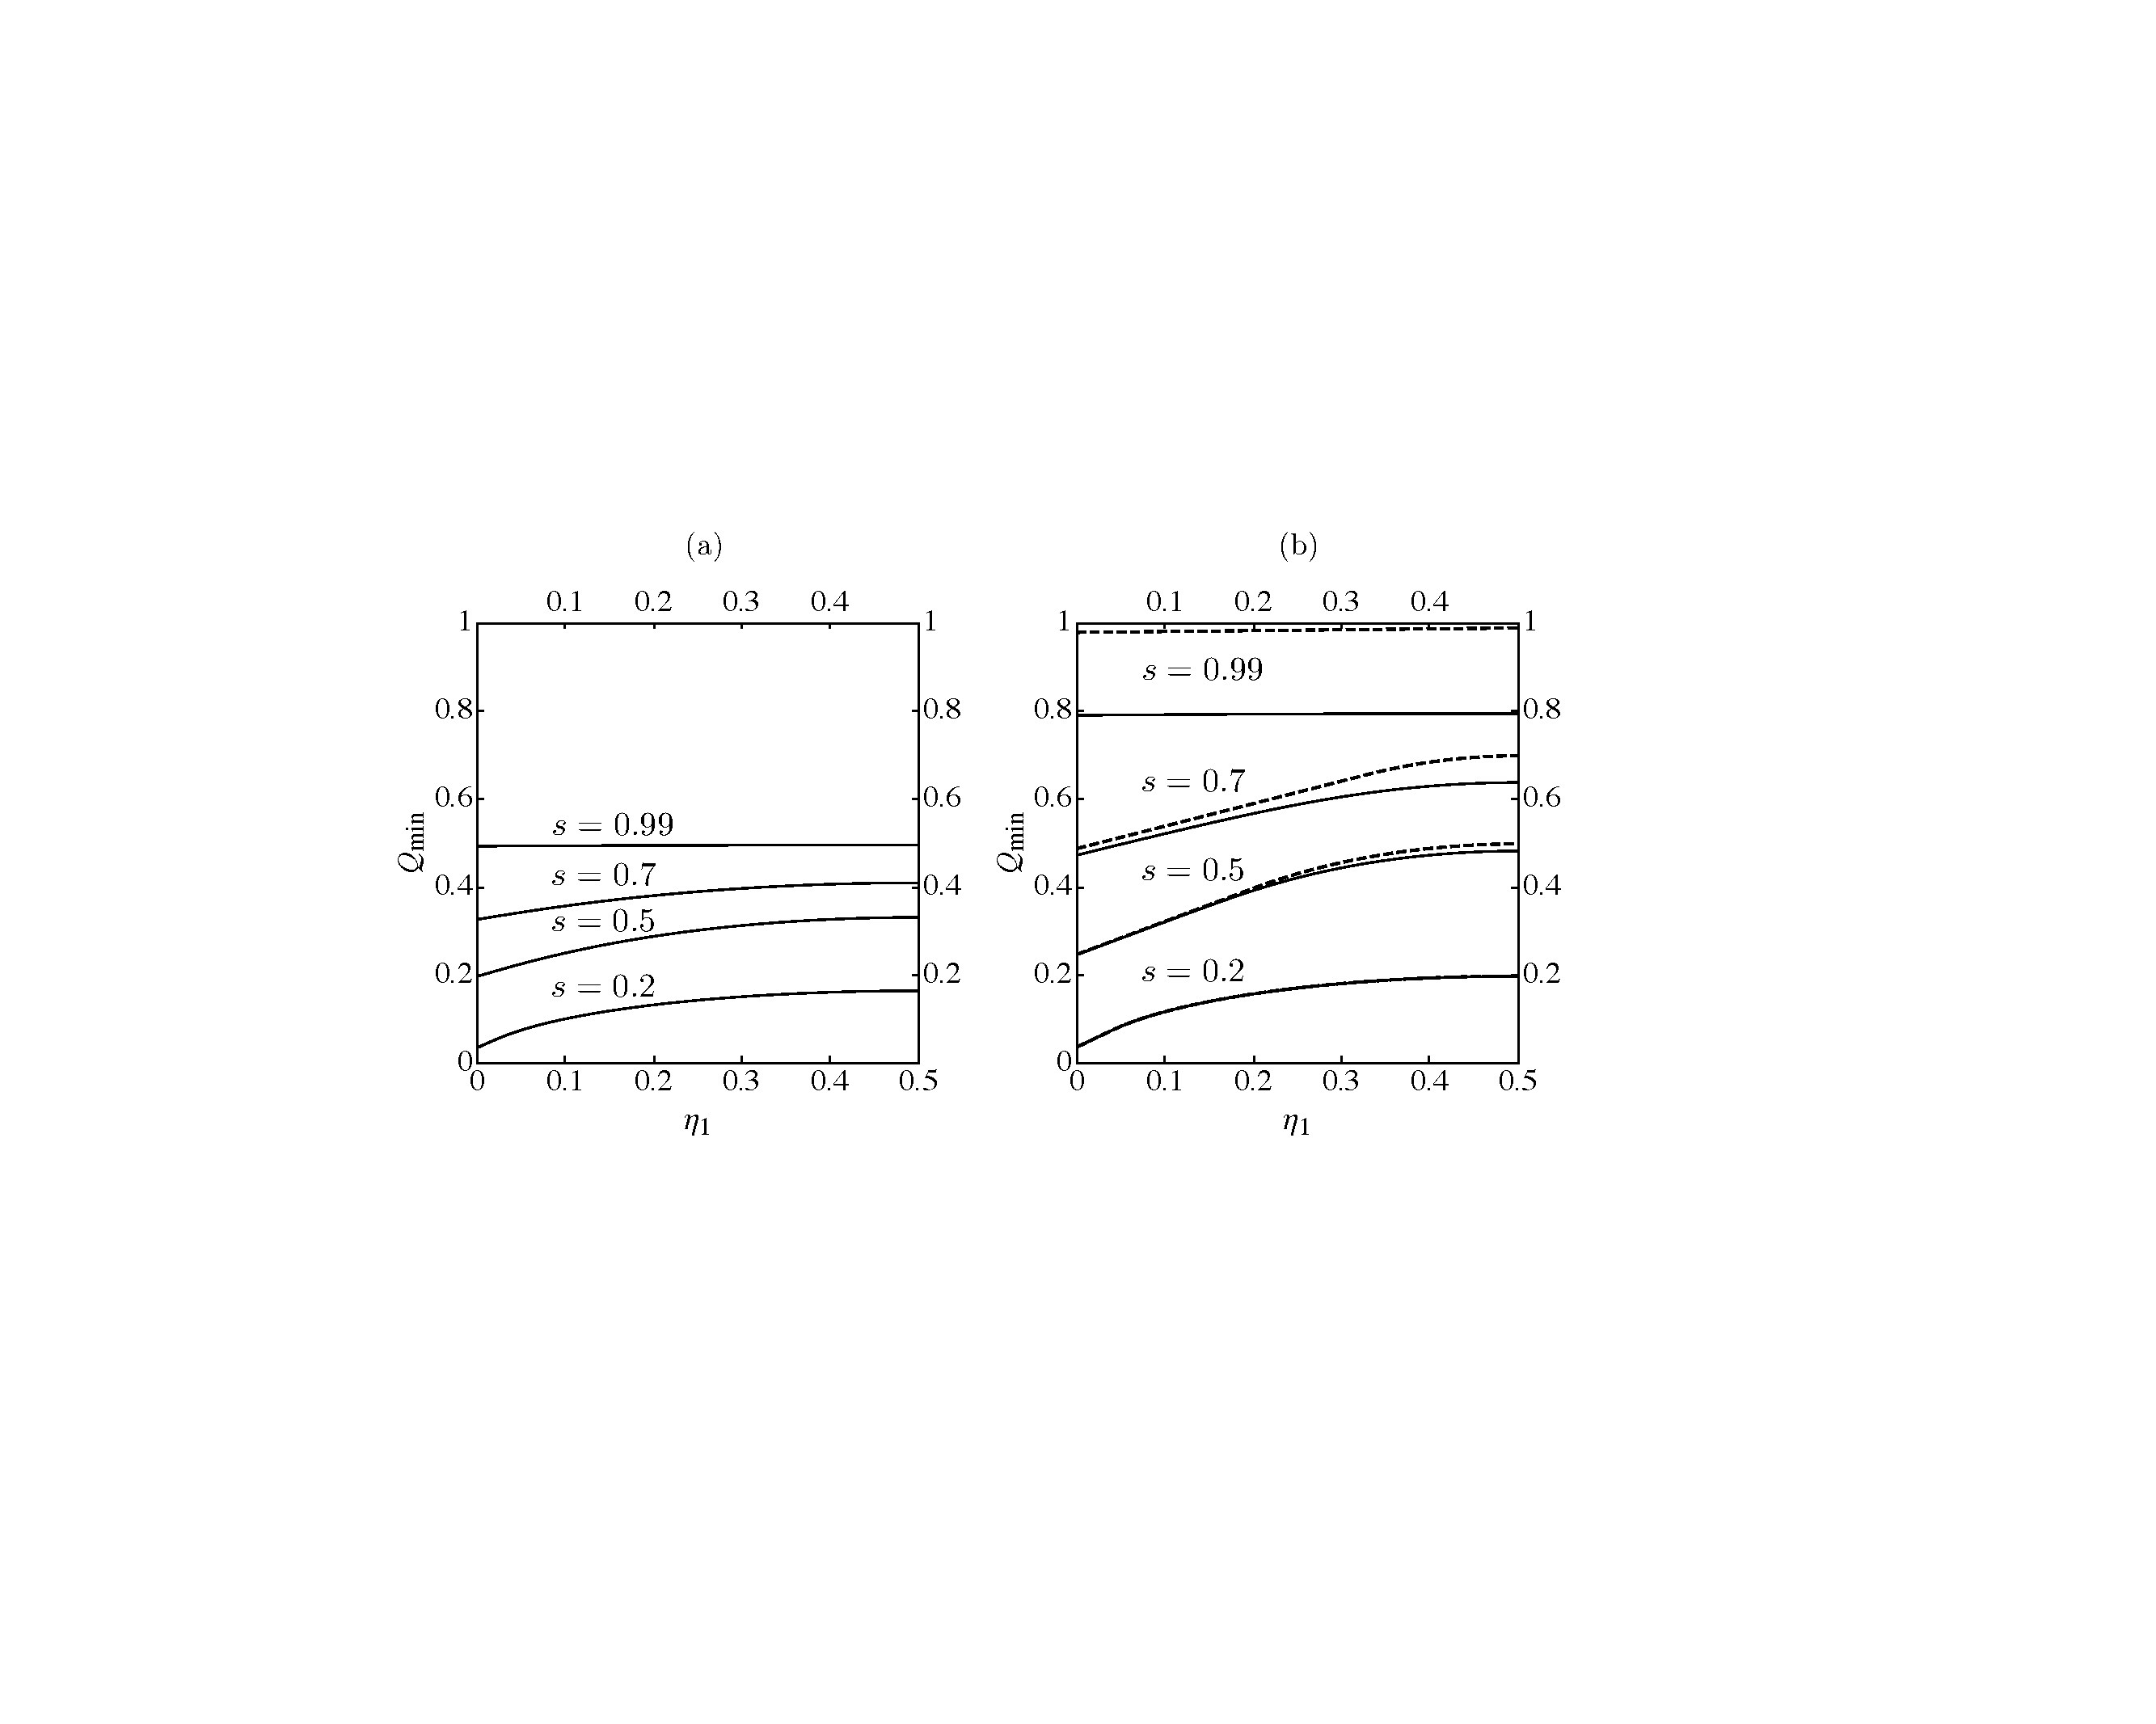
\includegraphics[width=26.7em]{Fig_3NC.pdf}\\
\end{array}%
$%
\caption{Fig (a) is plotted for $m=1$, $n = 2$ and Fig (b) for $m =1$, $n = 5$.  The dotted lines in (b) are the optimal UD solutions for the  same parameters.}
\end{figure}
\end{frame}
%%%%%%%%%%%%%%%%%%%%%%%%%%%%%%%5
%%%%%%%%%%%%%%%%%%%%%%%%%%%%%%%%%%%%%%%%%%%%%%%%%%%%%%%%%%%%%%%%%5
\subsection{Intermediate Cloning}
\begin{frame}
In between the two strategies we want approximate clones probabilistically:
\begin{eqnarray}
U \ke{\psi_1^M} \ke 0 = \sqrt{p_1} \ke {\phi_1} \ke 1 + \sqrt{q_1} \ke 0\\
U \ke{\psi_2^M} \ke 0 = \sqrt{p_2} \ke {\phi_2} \ke 1 + \sqrt{q_2} \ke 0 .
\end{eqnarray}

The unitarity constraint is $s^m = \sqrt{p_1 p_2} s' + \sqrt{p_1 p_2}$, the same as for separation.  However
our goal is to maximize the global fidelity for a fixed rate of failure.
\end{frame}
\begin{frame}
Chefles and Barnett solved the equal priors case in 1998, giving us the optimal global fidelity for N separable output states as 
\[F_{mn}  =\frac{1}{2\left(1-Q\right)}[(1-Q)+Q_{o}^{n}(Q_{o}-Q)+\]
\[\sqrt{(1-Q_{o}^{2n})\left[(1-Q)^{2}-(Q-Q_{o})^{2}\right]}].\]

This formula reduces to intermediate discrimination in the $n \rightarrow \infty$ limit.
As you may imagine the unequal priors case cannot be solved in the same manner.  
\end{frame}

%%%%%%%%%%%%%%%%%%%%%%%%%%%%%%%5
%%%%%%%%%%%%%%%%%%%%%%%%%%%%%%%%%%%%%%%%%%%%%%%%%%%%%%%%%%%%%%%%%5
\begin{frame}{Arbitrary Priors}
This takes two steps: first maximally separate the incoming states for a fixed rate of inconclusive result, 
\begin{itemize}
\item Step 1: State Separation
\end{itemize}
Optimally separate the incoming states $\left\{ \ke{\psi_{1}^{m}},\ke{\psi_{2}^{m}}\right\} $
with a fixed rate of inconclusive results $q_{i}$, then prepare states
$\left\{ \ke{\Psi_{1}},\ke{\Psi_{2}}\right\} $ with the
corresponding success probabilities. 

The incoming states are separated with a success probability $p_{i}$
and failed to separate the states with a failure probability $q_{i}$.
\end{frame}
%%%%%%%%%%%%%%%%%%%%%%%%%%%%%%%5
%%%%%%%%%%%%%%%%%%%%%%%%%%%%%%%%%%%%%%%%%%%%%%%%%%%%%%%%%%%%%%%%%5
\begin{frame}
\begin{itemize}
\item Step 2: Optimize Deterministic Fidelity
\end{itemize}
The resulting states are rotated in such a way that their average overlap with n copies of the original state is maximized. 
More precisely, for individual fidelities $F_i = |\bk{\psi_i^n}{\phi_i}|^2$ we want to maximize the global conditional fidelilty 
\[F = \frac{\eta_1 p_1 F_1 + \eta_2 p_2 F_2}{1-Q} = \tilde{\eta_1} F_1 + \tilde{\eta_2} F_2\]
Where we've also shown the resulting normalization.  This normalization means we can apply the deterministic fidelity result to this problem.
\end{frame}
%%%%%%%%%%%%%%%%%%%%%%%%%%%%%%%5
%%%%%%%%%%%%%%%%%%%%%%%%%%%%%%%%%%%%%%%%%%%%%%%%%%%%%%%%%%%%%%%%%5
\begin{frame}
The resulting fidelity expression,
\[F  = \frac{1}{2}\left[1+\sqrt{1-4\tilde{\eta}_{1}\tilde{\eta}_{2}\sin^{2}\left(\theta-\phi\right)}\right],\]
  has a remaining optimization under the square root, namely the term
\begin{equation*}
\Lambda =  \sqrt{p_{1}p_{2}}\sin\left(\theta-\phi \right).
\end{equation*}
can be written with optimal separation as
\begin{equation*}
\Lambda = \sqrt{1-s^{2n}}\left(s-u\right)-s^{n}\sqrt{1-s^{2}-2v+2sv}
\end{equation*}
where $u\equiv\sqrt{q_{1}q_{2}},\hspace{0.3cm}v\equiv\frac{1}{2}\left(q_{1}+q_{2}\right)$, 
are variables we introduced in the section on state separation.
\end{frame}
\begin{frame}
The solution can be parametrically expressed as
\begin{eqnarray}
Q\!&=&\!{(1\!-\!\Delta^2)(1\!-\!s^2)\!-\!\gamma_n\left(\Delta\cot\theta'\!+\!s\sqrt{1\!-\!\Delta^2}\right)^2\over2\left(1+\Delta\sin\theta'-s\sqrt{1-\Delta^2}\cos\theta'\right)},
\nonumber\\
%\zeta \!&=&\!{1\over\sqrt{1+\gamma_n}}\left[(1\!+\!\gamma_n)s\!+\!{\gamma_n\Delta\cot\phi\over\sqrt{1\!-\!\Delta^2}}\!-\!{Q\cos\phi\over\sqrt{1\!-\!\Delta^2}}\right]
\Lambda_{\rm min} \!&=&\!{(1\!+\!\gamma_n)\sqrt{1\!-\!\Delta^2}s\!+\!\gamma_n\Delta\cot\theta'\!-\!Q\cos\theta'\over\sqrt{1+\gamma_n}\sqrt{1\!-\!\Delta^2}},
\end{eqnarray}
where $\gamma_n=s^{2n}/(1-s^{2n})$, $\Delta=\eta_2-\eta_1$, and $\theta'$ is the parametrization variable.

\end{frame}
%%%%%%%%%%%%%%%%%%%%%%%%%%%%%%%5
%%%%%%%%%%%%%%%%%%%%%%%%%%%%%%%%%%
%%%%%%%%%%%%%%%%%%%%%%%%%%%%%%%5
%%%%%%%%%%%%%%%%%%%%%%%%%%%%%%%%%%
%%%%%%%%%%%%%%%%%%%%%%%%%%%%%%%5
%%%%%%%%%%%%%%%%%%%%%%%%%%%%%%%%%%
\section{Linear Optical Implementations}
\begin{frame}
Every unitary can be reduced into beam splitters and phase-shifters via the
Reck-Zeilinger algorithm.  This has been experimentally implemented for various protocols.

\begin{figure}[th]
\centering
$%
\begin{array}{c}
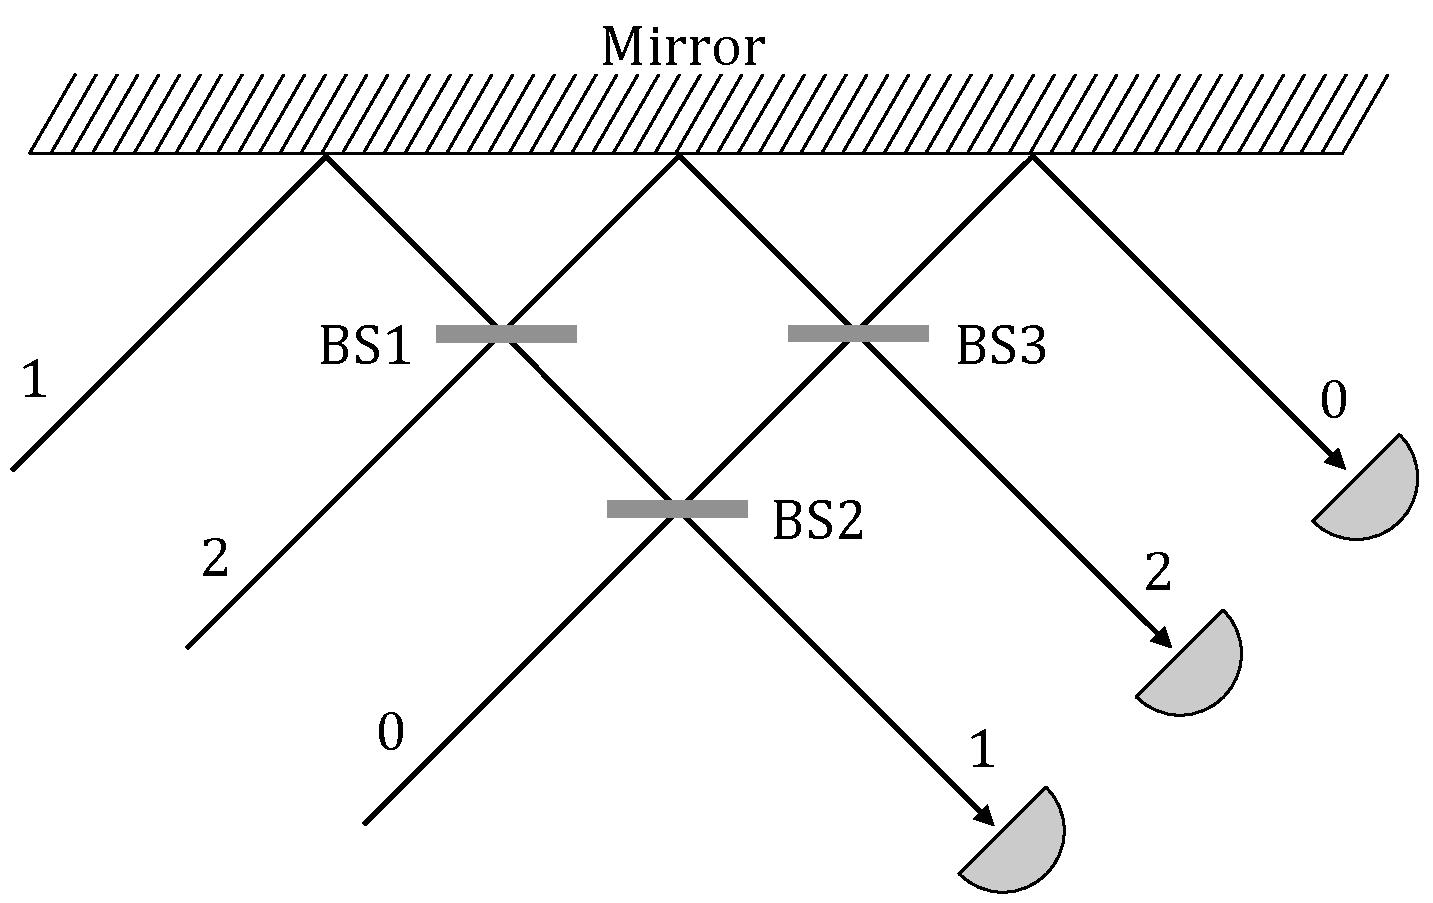
\includegraphics[height=5.5 cm]{Interferometer.pdf} \\

\end{array}%
$%

\label{fig:Graphs}
\end{figure}

\end{frame}
%%%%%%%%%%%%%%%%%%%%%%%%%%%%%%%5
%%%%%%%%%%%%%%%%%%%%%%%%%%%%%%%%%%%%%%%%%%%%%%%%%%%%%%%%%%%%%%%%%5
\begin{frame}{Approximate Probabilistic Cloning}
We can decompose the action of a probabilistic cloner into two steps,
first separate the states and then clone them to the desired copies.  We will show
this setup for equal prior probabilities and separable output states.
\end{frame}
%%%%%%%%%%%%%%%%%%%%%%%%%%%%%%%5
%%%%%%%%%%%%%%%%%%%%%%%%%%%%%%%%%%%%%%%%%%%%%%%%%%%%%%%%%%%%%%%%%5
\begin{frame}{Separation}
\begin{eqnarray}
U\ke {\psi_1} = \sqrt{p_1}\ke{\phi_1}+ \sqrt{q_1}\ke{0}\\
U\ke {\psi_2} = \sqrt{p_2}\ke{\phi_2}+ \sqrt{q_2}\ke{0}
\end{eqnarray}
where $\ke {\psi_1} = c_1 \ke{1} + s_1 \ke{2}$,
$\ke {\psi_2} = c_1 \ke{1} - s_1 \ke{2}$,
$\ke {\phi_1} = c_2 \ke{1} + s_2 \ke{2}$,
$\ke {\phi_2} = c_2 \ke{1} - s_2 \ke{2}$.
We sandwich equations (10) and (11) with basis bras, getting equation that we can solve for six of nine matrix elements:
\begin{eqnarray}
\br 0 U \ke {\psi_1} &=&c_1 U_{01} + s_1 U_{02} = \sqrt{q_1}\\
\br 1 U \ke {\psi_1} &=&c_1 U_{11} + s_1 U_{12} = c_2 \sqrt{p_1}\\
\br 2 U \ke {\psi_1} &=&c_1 U_{21} + s_1 U_{22} = s_2\sqrt{p_1}
\end{eqnarray}
\end{frame}
%%%%%%%%%%%%%%%%%%%%%%%%%%%%%%%5
%%%%%%%%%%%%%%%%%%%%%%%%%%%%%%%%%%%%%%%%%%%%%%%%%%%%%%%%%%%%%%%%%5
\begin{frame}
Using the optimal sucess rate 
\begin{equation}
p = \frac{\bk{\psi_1}{\psi_2}-1}{\bk{\phi_1}{\phi_2}-1},
\end{equation}
 we can choose the remaining elements to be
\begin{equation}
{}[U]=
\begin{pmatrix}\frac{c_2s_1}{c_1s_2}& \frac{\sqrt{s_2^2-s_1^2}}{c_1s_2} & 0\\
-\frac{\sqrt{s_2^2-s_1^2}}{c_1s_2} &\frac{c_2s_1}{c_1s_2} & 0 \\
0 & 0 & 1
\end{pmatrix}
\end{equation}
and only one beam splitter is needed to perform this operation.
\end{frame}
%%%%%%%%%%%%%%%%%%%%%%%%%%%%%%%5
%%%%%%%%%%%%%%%%%%%%%%%%%%%%%%%%%%%%%%%%%%%%%%%%%%%%%%%%%%%%%%%%%5
\begin{frame}{Deterministic Cloning}
The unitary transformation
for the second step is
\begin{eqnarray}
U\ke {\phi_1} \ke 0 = \ke{\xi_1}\ke{\xi_1}\\
U\ke {\phi_2} \ke 0 = \ke{\xi_2}\ke{\xi_2}
\end{eqnarray}
where 
$\ke {\xi_1} = c_3 \ke{1} + s_3 \ke{2}$ and
$\ke {\xi_2} = c_3 \ke{1} - s_3 \ke{2}$
Following a similar procedure we choose the basis states $ \ke {00}$,$ \ke {10}$,$ \ke {01}$, and$ \ke {11}$,
giving us the final unitary as 
\begin{equation}
{}[U]=
\begin{pmatrix} \frac{c_3^2}{c_2} &0 & 0 &\frac{s_3^2}{c_2}\\
0 &\frac{1}{\sqrt{2}} &\frac{1}{\sqrt{2}}&0 \\
0 &-\frac{1}{\sqrt{2}} &\frac{1}{\sqrt{2}}&0 \\
\frac{s_3^2}{c_2} & 0&0&\frac{c_3^2}{c_2}
\end{pmatrix}
\end{equation}
\end{frame}
%%%%%%%%%%%%%%%%%%%%%%%%%%%%%%%5
%%%%%%%%%%%%%%%%%%%%%%%%%%%%%%%%%%%%%%%%%%%%%%%%%%%%%%%%%%%%%%%%%5
\begin{frame}
This is clearly the action of two separate beam splitters $M_{14}$ and $M_{23}$ such that $U = M_{14} \cdot M_{23}$ where

\begin{eqnarray}
{}[M_{14}]=
\begin{pmatrix}\frac{c_3^2}{c_2} &0 & 0 &\frac{s_3^2}{c_2}\\
0&1&0&0\\
0&0&1&0\\
\frac{s_3^2}{c_2} & 0&0&\frac{c_3^2}{c_2}
\end{pmatrix}, \quad
{}[M_{23}]=
\begin{pmatrix}1&0&0&0\\
0&\frac{1}{\sqrt{2}} &\frac{1}{\sqrt{2}} &0 \\
0&-\frac{1}{\sqrt{2}} & \frac{1}{\sqrt{2}}&0\\
0&0&0&1
\end{pmatrix}
\end{eqnarray}
Since this last step is deterministic cloning we have the relationship between the overlaps as $ \bk {\phi_1}{\phi_2} = \bk {\xi_1}{\xi_2}^2$.  This leads to the relation $s_2^2 = 2 c_3^2 s_3^2$ and $c_3^2 = \frac{1}{2} \pm \sqrt{1-2s_2^2}$, resulting inthe $M_{23}$ beam splitter being just a 50-50 beam splitter.
\end{frame}













\section*{Thank you}

\begin{frame}{Thank you}

  % Keep the summary *very short*.
  \begin{itemize}
  \item
    Thank you
 
 
  \end{itemize}
  \end{frame}


% All of the following is optional and typically not needed. 
\appendix
\section<presentation>*{\appendixname}
\subsection<presentation>*{For Further Reading}

\begin{frame}[allowframebreaks]
  \frametitle<presentation>{For Further Reading}
    
  \begin{thebibliography}{10}
    
  \beamertemplatebookbibitems
  % Start with overview books.

  \bibitem{Author1990}
    A.~Author.
    \newblock {\em Handbook of Everything}.
    \newblock Some Press, 1990.
 
    
  \beamertemplatearticlebibitems
  % Followed by interesting articles. Keep the list short. 

  \bibitem{Someone2000}
    S.~Someone.
    \newblock On this and that.
    \newblock {\em Journal of This and That}, 2(1):50--100,
    2000.
  \end{thebibliography}
\end{frame}

\end{document}


